\documentclass[letterpaper, 10 pt, conference]{ieeeconf}  

\IEEEoverridecommandlockouts                             
\overrideIEEEmargins

\usepackage{graphics} 
\usepackage{graphicx}
\usepackage{epsfig} 
\usepackage{mathptmx} 
\usepackage{times} 
\usepackage{amsmath} 
\usepackage{amssymb}  
\usepackage{makeidx}
\usepackage{float}
\usepackage{balance}
\usepackage{url}
\usepackage[hidelinks]{hyperref}
\usepackage{cite}
\usepackage{flexisym}
\usepackage{chngcntr}
\usepackage{amsmath}
{
%      \theoremstyle{plain}
      \newtheorem{assumption}{\textbf{Assumption}}
      \newtheorem{definition}{\textbf{Definition}}
      \newtheorem{proposition}{\textbf{Proposition}}
      \newtheorem{lemma}{\textbf{Lemma}}
      \newtheorem{theorem}{\textbf{Theorem}}
}
\DeclareMathOperator*{\maxi}{max}
\DeclareMathOperator*{\mini}{min}

%----------------------------------------------

\title{\LARGE \bf Cooperative Mobile Manipulation without Explicit Communication}

\author{George P. Kontoudis
\thanks{This work was submitted on 02/05/17 and is part of the project for the class AOE5984-Cyber-Physical Systems \& Distributed Control, offered by Prof. Kyriakos Vamvoudakis, \url{kyriakos@vt.edu}}
\thanks{G. Kontoudis is with the Mechanical Engineering Department, Virginia Polytechnic Institute and State University, Blacksburg, VA, 24060, USA, \url{gpkont@vt.edu}}}

\begin{document}
\maketitle
\thispagestyle{empty}
\pagestyle{empty}

%----------------------------------------------

\begin{abstract}
A solution for the cooperative mobile manipulation problem of a group of N robots is presented. The main contribution of this methodology lies in the utilization of local information for robot coordination, without explicit communication. Local information for motion coordination is achieved through force feedback. The object's translational and rotational motion can be efficiently controlled. The proposed methodology can alter the leader either with a robot or with a human. The efficacy of the proposed method is verified through simulations, considering force analysis of agents.   
\end{abstract}

\normalsize{\bf\small\emph{Index Terms:} mobile manipulation, cooperative control, consensus algorithms}  

%----------------------------------------------

\section{Introduction}\label{intro}

A multi-robot manipulation algorithm which integrates local information is presented \cite{wang2016force}. Multi-robot cooperation can be accomplished without explicit communication, but only with local information. The suggested local information is force feedback, gathered and processed individually from each robot. The leader can be either a robot or a human, but in each case operates as the dominant agent of motion planning. The desired trajectory is imposed by the leader while the followers regulate their forces according to the leader's amplitude and direction.   

Multi-agent networks with communication face several problems. Communication is usually very noisy, demands high computational power, deals with uncertainty and in some cases might get vanished. The relationship of the number of nodes with communication complexity is proportional, that means for large networks a major issue lies in communication between agents. An interesting approach is to neglect communication between agents and design a strategy to attain consensus through force feedback for each agent locally. In this way, communication problems can be fully confronted, so update of the network can be managed at any time. 

Robotic manipulation is an emerging field for many decades. In case we consider each robot as a finger, and each local attachment point as a contact point, then we get similar structure and properties with multi-fingered grasping and manipulation tasks \cite{murray1994mathematical}, \cite{prattichizzo2016grasping}. However, after efficiently grasp an object with several robots, we need to maintain a stable grasp by applying effective caging strategies \cite{fink2008multi}, \cite{pereira2004decentralized}. Transferring objects with multiple robots demands an untrivial motion planning approach \cite{donald1997information}, \cite{rus1995moving}. Multi-agent consensus is a similar field, which is employed to develop force consensus between agents without communication \cite{jadbabaie2003coordination}, \cite{olfati2007consensus}, \cite{ren2005consensus}. The whole procedure is bio-inspired from ant colonies, as it recognized that ants have a specific leader when they cooperate to move objects \cite{gelblum2015ant}. Moreover, ants do not explicitly communicate, but instead they employ object's vibration and/or deformation to coordinate their motion \cite{mccreery2014cooperative}. 

In this project we implement 2D planar motion of robots and object $Q \in \mathbb{R}^2$. We consider $N$ robots of a set $R_i$, with $i=1, \hdots ,N$, where $R_1$ is always the leader, and the other robots are the followers. Therefore, the leader drives the system by following a desired trajectory, that is unknown to the rest robots. Moreover, any form of communication is forbidden along agents. The motion control algorithm using force feedback consists of two steps. First, the followers need to recognize the leader's force magnitude and direction, by employing force feedback. Then, the followers have to cooperate and provoke a resultant force in the same direction and with larger amplitude.  Furthermore, two different force analyses were occurred as object shape and mass may be varied. In the first case, an analysis of drugging low-weight objects is presented, while in the second case an analysis for heavy-weight objects, which assumed to be placed on a moving platform, is provided. 

Difficulties that we expect to face are to determine whether this technique is accurate and robust in terms of following the desirable trajectory of the leader and not damage the object. Then, the performance of the proposed technique should exceed the performance of cooperative multi-robot systems with explicit communication. Simulation of the problem is ideal to be implemented, but it also accounts of avoiding collision for every agent. Therefore, we study a cooperative mobile manipulation technique without communication, by simulating the force magnitude and tracking the direction of the leader from the follower agents.

The remainder of this report is organized as follows. Section \ref{pf} discusses the problem formulation. The efficacy of the proposed methodology is assessed in Section \ref{sim} by a set of simulations. Finally, Section \ref{concl} provides the conclusions of the studied methodology and gives directions for future work.

%----------------------------------------------

\section{Problem Formaulation}\label{pf}
In this section we formulate the proposed methodology for planar cooperative manipulation without communication, using force feedback. We study 2 different force feedback cases. First, we deal with the manipulation of lightweight objects that can be efficiently moved from a small number of robots. This methodology studied in   \cite{wang2016force}, \cite{wang2016kinematic} and characterized as constant boost force (CB-ANTS). Next, we analyze the condition of heavyweight objects where the robots lift and drag the object for its motion in 2-$D$ space as in \cite{wang2015multi}, \cite{wang2016force}. The later method refered as proportional force (P-ANTS). The reason that these two methodologies were discriminate is keen on friction. The friction for the motion of rigid bodies is divided in two terms, the static and the kinetic. Static friction is proportional to the applied force and dominates while the rigid body is not moving. The maximum value of static friction coefficient emerges just before slipping. In case that the applied forces overcome the static friction the motion of the object appears. While the object is sliding the only friction that applies is the kinetic. In most cases the coefficient of static friction is greater than the coefficient of kinetic friction \cite{tipler2007physics}. If the object is lightweight we can easily produce drag forces to overcome the static friction, but when the object is heavyweight the problem becomes nontrivial. Therefore the methodology suggests for heavyweight objects to lift and drag the objects. In such case, the sliding friction cannot express our system because the object is rolling. The rolling friction is significantly lower than the  kinetic friction while the object is rolling on the ground. While the the object is on the rolling device the friction is proportional to the velocity and not the force. Furthermore, we do not have to deal with the static friction of the object. Depending on the weight, similar techniques are followed by humans to relocate objects. 

\subsection{Rigid Body Dynamics}\label{rbd}
In this section we study the object as rigid body and the relevant dynamics are presented. Given the object's mass $M$ in ($kg$), and acceleration of gravity $g$ in $m/s^2$. The applied forces of the robots are indicated as $\{ F_1, F_2, \hdots, F_N \}$ in $N$, and the linear velocity of the object as $v$ in $m/s$. We assume that the coefficient of kinetic friction $\mu_k$ is constant and its direction is always opposed to the object's velocity vector. Moreover, the coefficient of static friction $\mu_v$ is proportional to the object's applied force. The translational motion of the object is subject to the second law of Newton. The object's dynamics for translational movement can be described as 
\begin{equation}
M\dot{v}=\sum_{i=1}^N F_i-\mu_{k}Mg\frac{v}{||v||}-\mu_v v.
\end{equation}

In case we drag the object (F-ANTS) we can eliminate the static friction because we assume that the object is moving, and thus we discretize by employing Euler's method 
\begin{equation}\label{dod}
M\frac{v_{t+1}-v_t}{\Delta t}=\sum_{i=1}^N F_i(t)-\mu_kMg\frac{v_t}{||v_t||}.
\end{equation}
For heavyweight objects we only consider the static friction of the rollers, which yields 
\begin{equation}\label{roldyn}
M\dot{v}=\sum_{i=1}^N F_i-\mu_v v.
\end{equation}

In this study we assume that the object's mass, the coefficient of kinetic friction, the coefficient of static friction, the acceleration of gravity, and the number of robots, that take part to the cooperative manipulation of the object, are given for all robots.
\begin{assumption}\label{as1}
\textit{All robots have information about the exact values of $M$, $\mu_k$, $\mu_v$, $g$, $N$.}
\end{assumption}
 
\subsection{Rotational Dynamics}\label{rd}
In this section the rotational dynamics of the object and the local measurement, that the robots can gather about the object's motion, are discussed. Measurement of the object's velocity in center of mass (CoM) is not feasible to be taken in practice. However we can get information from the robot about the translational velocity and the angular velocity at the contact point. \vspace{.2cm}
\begin{assumption}\label{as2}
\textit{The leader have information about the angular velocity of the object and applies a torque $T_1$.} \vspace{.2cm}
\end{assumption}
Given the object's moment of inertia $J$ in $kg-m^2$, the angular velocity $\omega$ in $rad/s$, and under the Assumption \ref{as2} we can derive the overall rotational dynamics of the studied object as follows
\begin{equation}\label{rotDyn1}
J\dot{\omega}=T_1 +\sum_{i=2}^{N}r_i\times F_i-T_f,
\end{equation}
where $T_f$ is the torque related with the static friction, $\sum_{i=2}^{N}r_i\times F_i$ is the torque produced by the follower robots, $r_i$ is the vector from the object's center of mass to the contact point of the $i$-robot,  and $T_l$ is the torque imposed by the leader robot.\vspace{.2cm}
\begin{proposition}\label{pr1}
\textit{For any rigid body object with an arbitrary shape in a planar region $Q \in \mathbb{R}^2$ the frictional torque caused by the static friction is given as}
\begin{equation}
T_f=-\frac{\mu_{\nu}}{M}J\omega.
\end{equation} \vspace{.2cm}
\end{proposition}
As a result the overall rotational dynamics of equation \ref{rotDyn1} under Proposition \ref{pr1} yields
\begin{equation}\label{rotDyn2}
J\dot{\omega}=T_1 +\sum_{i=2}^{N}r_i\times F_i-\frac{\mu_{\nu}}{M}J\omega.
\end{equation}

Since we study objects as rigid bodies the only feasible contact points for the robots to grasp the object are at the object's perimeter. Furthermore, if the mass of the rigid body is not evenly distributed it becomes difficult to get the exact position of the object's center of mass. The information that we can get are the measurements of contact points and the translational velocity of the object. The local motion measurements include the velocity and the acceleration of the robot at the contact point, that can be written in global reference of the object's center of mass 
\begin{equation}
v_i=v_c +\omega \times r_i,
\end{equation}
\begin{equation}
\dot{v}_i=\dot{v}_c +\dot{\omega }\times r_i+\omega \times (\omega \times r_i),
\end{equation}
where $v_i$, $\dot{v_i}$ are the velocity and the acceleration at the contact point respectively. Since, that contact points to the object are fixed, Coriolis acceleration does not exist. An important issue that arises with the object's rotation is that each robot has a different motion measurement, that prevents for effective analysis. Thus, the local measurement study is not reproduced with simulations in this project. In case that we did not have time restrictions we could perform experiments with real robots and gather data to validate the efficacy of the suggested methodology.

An important aspect for the efficiency of the proposed methodology deals with the position of the contact points. To guarantee the performance of the proposed methodology Assumption \ref{as3} should be made.\vspace{.2cm}
\begin{assumption}\label{as3}
\textit{The contact points are centrosymmetric with respect to the object's center of mass, so $\sum_{i-1}^{N}r_i=0$.} \vspace{.2cm}
\end{assumption}
Under Assumption \ref{as3} and if the forces of all robots converge to a value the second term of equation \ref{rotDyn2} is vanished. In practice centrosymmetry assumption is difficult to be achieved, because we do not have knowledge about the exact center of mass for the studied objects.

\subsection{Constant Boost Force (CB-ANTS)}\label{cb}
In this section we present the constant boost force (CB-ANTS) case, where the robots drag the object through the desired trajectory to the goal position. Kinetic friction is the dominant friction and we assume that the coefficient of kinetic friction has a constant value. First, the methodology is based on the global information of the object's velocity at the center mass. Next, the exploitation of only local information at the contact points of each robot is employed to study a force feedback controller.

The follower's force feedback controller is designed as follows
\begin{equation}\label{cbfc}
F_i^c=\frac{\mu_k Mg}{N}\frac{v^c}{||v^c||}, \hspace{.2cm} i=\{ 2,3,\hdots , N\},
\end{equation}
where $i$ are the follower robots, $v^c$ is the velocity of the object at the center of mass, and $\hat{v}^c=\frac{v^c}{||v^c||}$ is the unit tangent vector that gives us the direction of the force. This force feedback controller was selected because it combines the velocity of the object at the center of mass which provide information for the leader's motion intention respectively. Moreover, the restriction of follower's forces result the dominance  of the leader's force.

The leader's force feedback controller is designed as follows
\begin{equation}\label{cblc}
F_l^l= f_d \frac{v_d^l}{||v_d^l||}= K_pmax\{ ||v_d^l||-||v^l||,0 \}\frac{v_d^l}{||v_d^l||},
\end{equation}
where $v_d^l$, $v^l$ is the desired and the current velocity of the leader robot respectively, $K_p$ is the proportional gain, and $\hat{v}_d=\frac{v_d^l}{||v_d^l||}$ is the unit tangent vector of the desired force of the leader robot. The max function is utilized to track the leader's velocity and switch to $0$ when it reaches the desired value in order to maintain the correct direction. The overall goal of the leader robot force feedback controller is to steer the object through a specific trajectory to the goal position.

We rely on Lemma \ref{lem1} to achieve consensus. \vspace{.2cm}
\begin{lemma}\label{lem1}
\textit{Given a discrete system $v_t$ is calculated as follows
\begin{equation}
v_{t+1}=\alpha_1 w+\beta_1 v_t,
\end{equation}
where $w$ is a vector with constants, $\{ \alpha_t|\alpha_t \geq 0, a_0^2+a_1^2+\hdots +a_t^2 \neq 0 \}$, and $\{ \beta_t|0<\beta_t<1 \}$. Then, $v_t$ converges to the direction of $w$ at $t \rightarrow \infty$ with a constant rate
\begin{equation}
v_t \rightarrow \gamma w,
\end{equation}
where $\gamma >0$ and has the form of
\begin{equation}
\gamma =\alpha_{t-1} + \beta_{t-1}\alpha_{t-2}+\beta_{t-2}\beta_{t-1}\alpha_{t-3}+\hdots+\beta_{t-1}\hdots \beta_1\beta_0\alpha_0.
\end{equation}} \vspace{.2cm}
\end{lemma}
\begin{theorem}\label{thrm1}
\textit{In the constant boost force (CB-ANTS) case by employing equations \ref{dod}, \ref{cbfc}, \ref{cblc} all follower robots align to the leader's direction and converge to a boost consensus value 
\begin{equation}
\phi = (N-1)\frac{\mu_kMg}{N},
\end{equation}
with time step $0<\Delta t<N\frac{||v_t||}{\mu_kg}$. Moreover object's velocity converge to the leader's desired velocity.} \vspace{.2cm}
\end{theorem}
The dynamic equations that we utilize for the constant boost force (CB-ANTS) case are expressed as
\begin{equation}
v_{t+1}= \Bigg(1-\frac{\mu_k g \Delta t}{N||v_t||}\Bigg)v_t+ \frac{\Delta t K_pmax\{ ||v_d^l||-||v^l||,0 \}}{M ||v_d||}v_d
\end{equation}
Note that the leader robot has to have specific force abilities to steer the object. That reveals the leader robot's demanding force, which needs to be at least above the value $\mu_kMg/N$. 

Since the convergence is guaranteed, the study of the convergence rate is mandatory to evaluate the performance of the methodology.\vspace{.2cm}
\begin{theorem}\label{thrm2}
\textit{Converge of follower's forces to the leader's force is succeeded with an exponential fast rate.} \vspace{.2cm}
\end{theorem}

\subsection{CB-ANTS using Local Measurements}\label{cblm}
In this section the analysis of constant boost force (CB-ANTS) with local measurements is presented. We want to converge in a specific value as we did in the previous case, so we want to keep the validity of Theorem \ref{thrm1}. Local motion measurements include velocity and acceleration of the object at robot contact points. Follower's controller by employing local measurements takes the form of
\begin{equation}
F_i=\frac{\mu_kMg}{N}\frac{v_t+\omega_t\times r_i}{||v_t+\omega_t\times r_i||},
\end{equation}
while the leader's force feedback controller has the same form as in equation \ref{cblc}. Since the follower's controller changed, the object's dynamic equation needs to alter respectively, so the constant boost force (CB-ANTS) with local measurements object's dynamics are given by
\begin{equation*}
v_{t+1}= \frac{\Delta t}{M}f_d\frac{v_d}{||v_d||}+\sum_{i=2}^N \bigg(\frac{\mu_k g \Delta t}{N||v_t+\omega_t \times r_i||} \bigg) \omega_t \times r_i+
\end{equation*}
\begin{equation}\label{cblmd}
+\Bigg(1+\sum_{i=2}^N \frac{\mu_k g \Delta t}{N||v_t + \omega_t \times r_i||}-\frac{\mu_k g \Delta t}{||v_t||}\Bigg)v_t.
\end{equation}
The first term stands for the control input in our system which is the desired velocity of the leader $v_d$. We would like to eliminate the second term, because it stands for the disturbing term. The third term is the internal dynamics of the studied object. In order to stabilize the system we desire the last term to be bounded as $|a|<1$.\vspace{.2cm}
\begin{theorem}\label{thrm3}
\textit{A sufficient condition to maintain theorem \ref{thrm1} is to bound the angular velocity as follows
\begin{equation}
||\omega_t||<\frac{||v_t||}{N||r_m||},
\end{equation}
where $m$ denotes the maximum radius value of the center of mass to the contact point, $m=\max\limits_{i}||r_i||$, $i=2,\hdots,N$.
} \vspace{.2cm}
\end{theorem}
As one can notice, convergence for constant boost force (CB-ANTS) with local measurements might achieved even when Theorem \ref{thrm3} is violated. As a result the constraint in Theorem \ref{thrm3} should be treated as a reference value.\vspace{.2cm}
\begin{theorem}\label{thrm4}
\textit{In case we guarantee centrosymmetric contact points, follow Theorem \ref{thrm3}, and utilize more than three robots  $N>3$ then we can restrict the disturbing factor in equation \ref{cblmd} as
\begin{equation}
\Bigg| \Bigg| \sum_{i=2}^N \Bigg( \frac{\mu_k g \Delta t}{n||v_t+ \omega_t \times r_i||} \Bigg)\omega_t \times r_i \Bigg| \Bigg|< \frac{\mu_k g \Delta t}{N} \Bigg( \frac{2N-1}{N^2-N} \Bigg)
\end{equation}
} \vspace{.2cm}
\end{theorem}
Notice that the inequality is direct related to a scaling factor $(2N-1)/(N^2-N)$. This scaling factor reveals that as we increase the number of robots the disturbing term in equation \ref{cblmd} is scaled down exponentially as depicted in figure \ref{scaling}.
\begin{figure}[!h]
	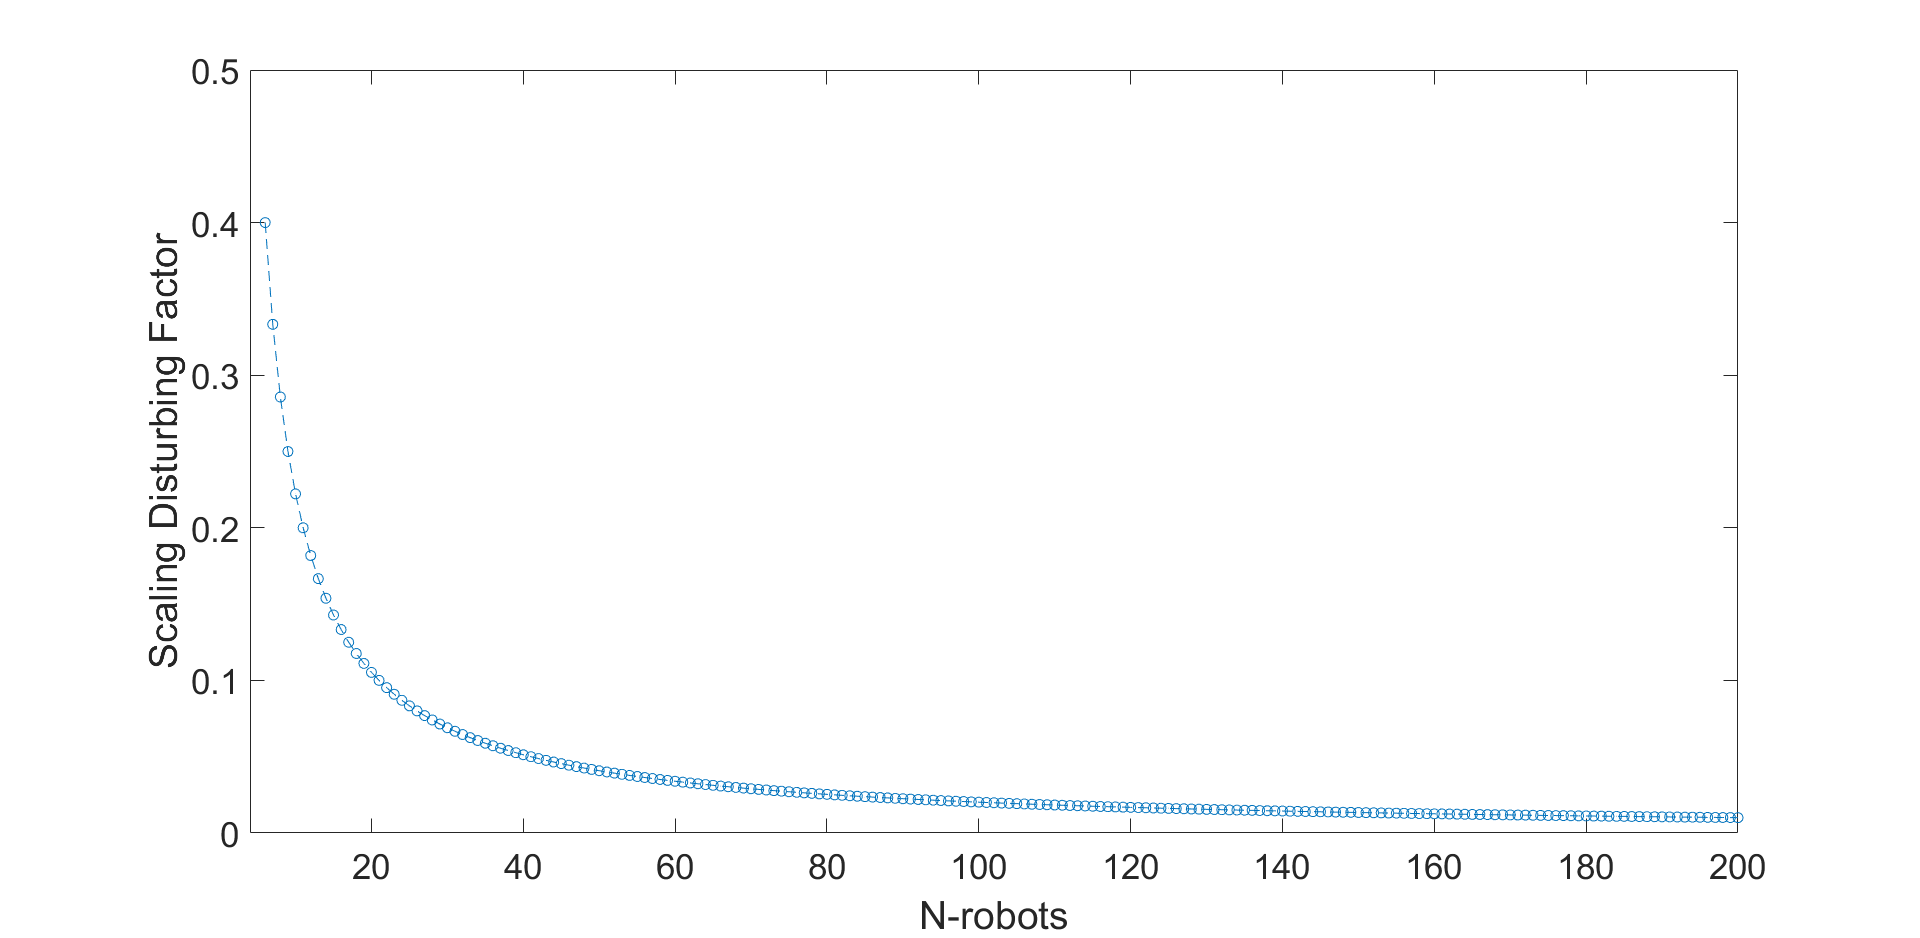
\includegraphics[width=.53\textwidth]{figures/scalingFactorDisturbance.png}
	\centering
	\caption{Disturbing factor of equation \ref{cblmd} decreases exponentially while the number of robots, taking part to the cooperative manipulation, increases.}
	\label{scaling}
\end{figure}

\subsection{Proportional Force (P-ANTS)}\label{pants}
In this section the second case of proportional force (P-ANTS) is presented for heavyweight objects. In this case rolling (viscous) friction of the rolling device is the only friction that occurs in the system, because the object is lifted in order to be transferred to the desired position. Rolling (viscous) friction of the rolling device, is significantly lower than the kinetic friction of the previous case. Note that an effort to lift the object is demanded, but is still lower than the force required for the object's motion when it lays on the floor. This methodology based on consensus analysis \cite{olfati2007consensus}, \cite{olfati2004consensus}. The consensus protocol commonly used for flocking is given by
\begin{equation}\label{consensus}
\dot{F}_i=\sum_{j \in N_i} (F_j - F_i)=\sum_{j \in N_i}F_j-NF_i,
\end{equation}
where $N_i$ is the interaction neighborhood, $F_j$ are the forces of the neighbors, $F_i$ is the force of the studied robot, and $N$ is the number of robots. The result implies an N-complete graph and since regular communication methodologies are not employed, we need another approach. By substituting equation \ref{roldyn} we get
\begin{equation}\label{pantsdyn}
\dot{F}_i=M\dot{v}+\mu_v v-NF_i.
\end{equation} 
Therefore, equation \ref{pantsdyn} assure force consensus without explicit communication, while the leader does not change its force and in case we have the object's velocity and acceleration at the center of mass.\vspace{.2cm}
\begin{proposition}\label{pr2}
\textit{Using the force controller in equation \ref{pantsdyn} and assuming that the leader robot maintain its initial force all the follower robots converge asymptotically to the leader's force value
\begin{equation}
\lim\limits_{t \rightarrow \infty} F_i(t)=F_l(0), \hspace{.3cm} i\in \{2, \hdots, N\}
\end{equation}} \vspace{.2cm}
\end{proposition}
As a result of Proposition \ref{pr2} the total force of the system as $t \rightarrow \infty$ becomes $NF_l$.\begin{theorem}\label{thrm5}
\textit{Using equation \ref{pantsdyn} the dynamic equations take the form of
\begin{equation}
\dot{\eta}=-\eta+F_l
\end{equation}
\begin{equation}
F_s=(N-1)\eta+F_l,
\end{equation}
where $F_l$ is the leader's force and the input, $\eta=(\sum_{i=2}^{N}F_i)/(N-1)$ is the average force of the followers and our state, and $F_s=\sum_{i=1}^N F_i$ is the total force and the output of our system.} 
\vspace{.2cm}
\end{theorem}
Using Theorem \ref{thrm4} we can derive the transfer function of the system as follows
\begin{equation}
\frac{F_s(s)}{F_l(s)}=\frac{s+N}{s+1}.
\end{equation}
Since the convergence is guaranteed, the study of the convergence rate is mandatory to evaluate the performance of the methodology.\vspace{.2cm}
\begin{theorem}\label{thrm6}
\textit{Convergence of follower forces to the leader's force is succeeded with an exponential fast rate, while the leader applies a constant force.} \vspace{.2cm}
\end{theorem}
The result of Theorem \ref{thrm6} is still valid for time dependent leader's force, but in such case we need to set $\dot{\tilde{F}}_l=F_l-\tilde{F}_l$.

\subsection{P-ANTS using Local Measurements}\label{pantslm}
In this section the analysis of proportional force (P-ANTS) with local measurements is presented. We want to converge to a specific value as we did in the previous case, so we want to keep the validity of Theorem \ref{thrm5}. Local motion measurements include velocity and acceleration of the object at robot contact points. Follower's controller by employing local measurements takes the form of
\begin{equation}\label{pantsdlm}
\dot{F}_i=(\sum_{j \in N}F_j-NF_i)-\frac{M}{J}r_i\times (\sum_{j\in N}r_j\times F_j),
\end{equation}
where the first term is similar to equation \ref{consensus}, and the next term is disturbance. The leader's torque was assumed to be negligible for many robots and thus was set to zero. Moreover, under Assumption \ref{as3} the centrifugal terms were eliminated.

The matrix form of equation \ref{pantsdlm} after some manipulation yields
\begin{equation}\label{mpants}
\dot{F}=\Bigg( -L_a-\frac{M}{J}R_a(t) \Bigg)F = -LF,
\end{equation}
where $F \in \mathbb{R}^{2N}$ is the vector of forces,  $L_a  \in \mathbb{R}^{2N\times 2N}$ is an extension of Laplacian matrix, $L$ is the Laplacian matrix, and $R_a(t) \in \mathbb{R}^{2N\times 2N}$ is the product of skew matrices. Notice that equation \ref{mpants} is focus only in 2D-space. 

Moreover under Assumption \ref{as3} the eigenvalues o Laplacian matrix are less or equal to zero only if 
\begin{equation}\label{mpantsBound}
\frac{M}{J}\sum_{i=1}^N||r_i||^2<N,
\end{equation}
which give us a bound regarding the number of robots $N$ with respect to the inertia matrix $J$, the mass of the object $M$, and the radius from the contact point to the center of mass of the object.
%----------------------------------------------

\section{Simulations and Results}\label{sim}
In this section we conduct simulations to verify the efficacy and robustness of the proposed methodology. We implement two set of simulations for both constant boost force (CB-ANTS) and proportional force (P-ANTS) cooperative mobile manipulation techniques. The first part of simulations uses a short number of robots and lightweight objects, while the second set deals with many robots and heavyweight objects. More information about the simulations can be found in the following link.
\begin{center}
\url{https://github.com/gkontoudis/VT-Courses}
\end{center}

\subsection{CB-ANTS Simulations}
For lightweight objects the methodology that proposed was the constant boost force (CB-ANTS). This technique requires to drag the object on the floor where the major type of friction is kinetic. The mass of the object that we employed for the simulations was $m=2kg$, the number of robots that took part to the cooperative motion was $N=20$. The maximum applied force of the leader could reach $F_l=0.96N$, while the followers could contribute up to $F_i=0.8N$. The kinetic friction was defined to $\mu_k=0.59$, and the maximum velocity of the robots was up to $v_c=0.3m/s$. It was found that a reliable proportional gain for this system was $K_p=6$. The path that was imposed from the leader was a rhombus (diamond). Time step was determined as of Theorem \ref{thrm1} to $\Delta t =0.3s$.
\begin{figure}[!h]
	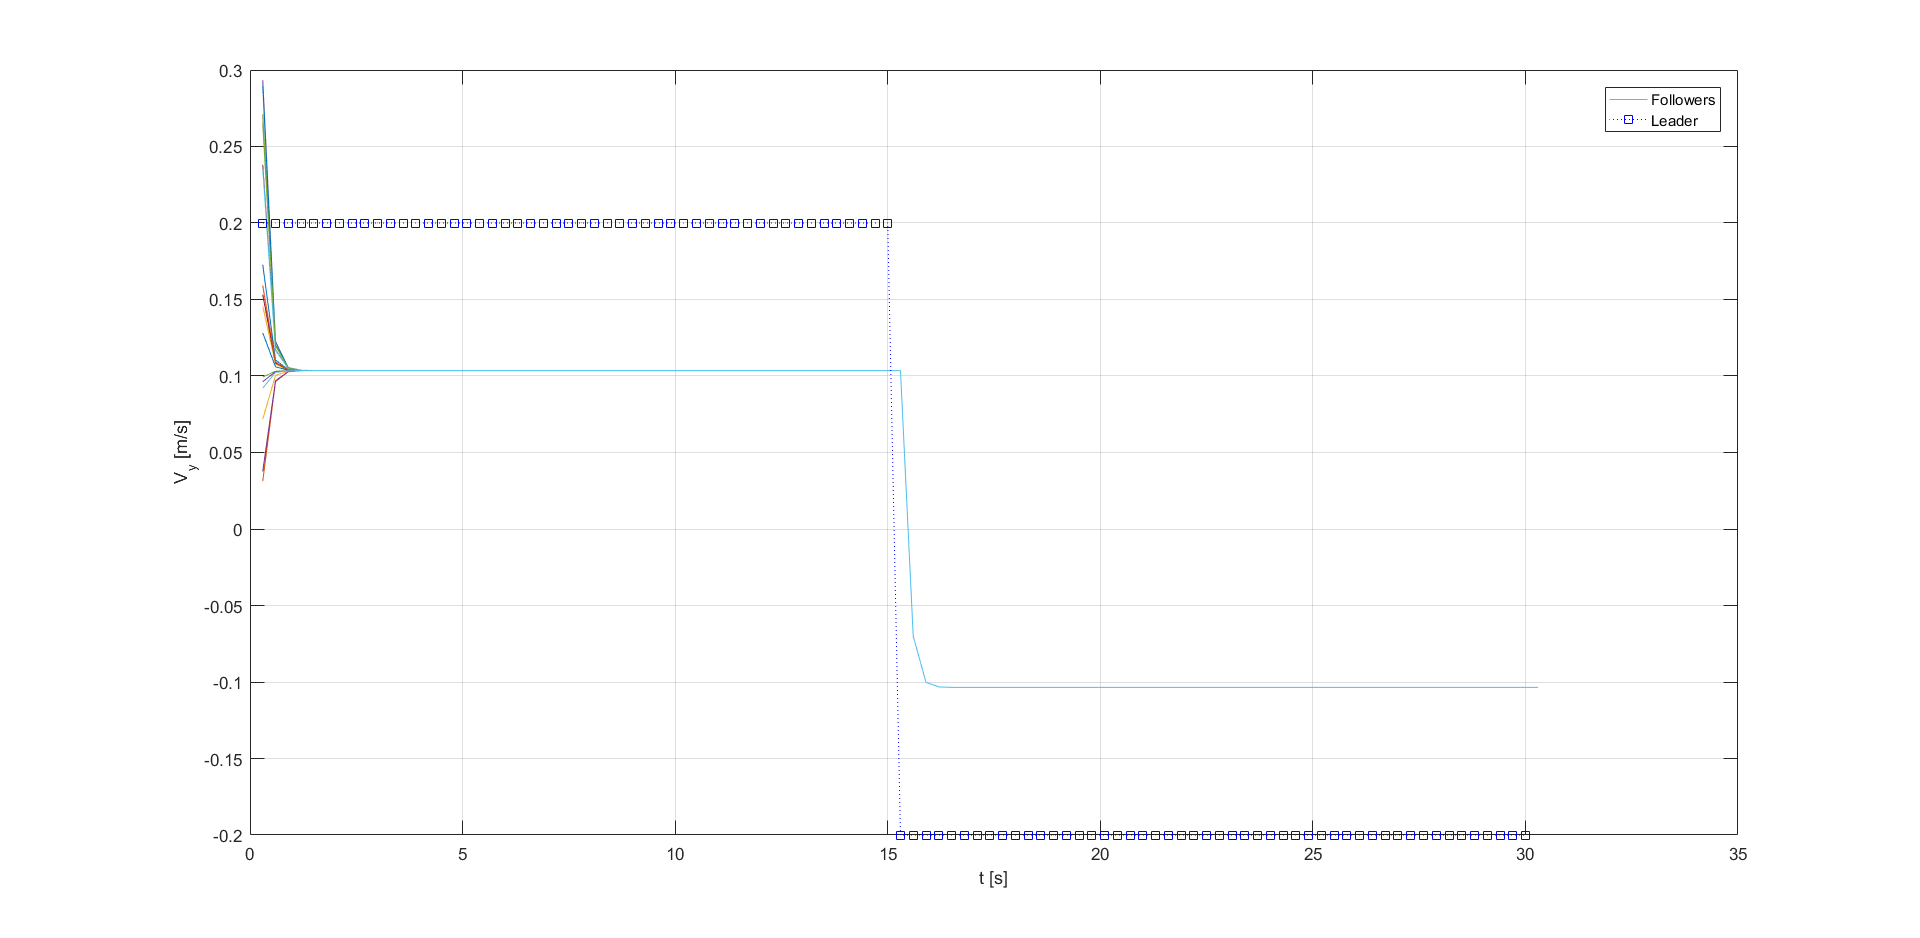
\includegraphics[width=.53\textwidth]{figures/CB_ANTS_Vy.png}
	\centering
	\caption{Velocities in y axis  $V_y$ using CB-ANTS with global measurements.}
	\label{fcbvy}
\end{figure}
\begin{figure}[!h]
	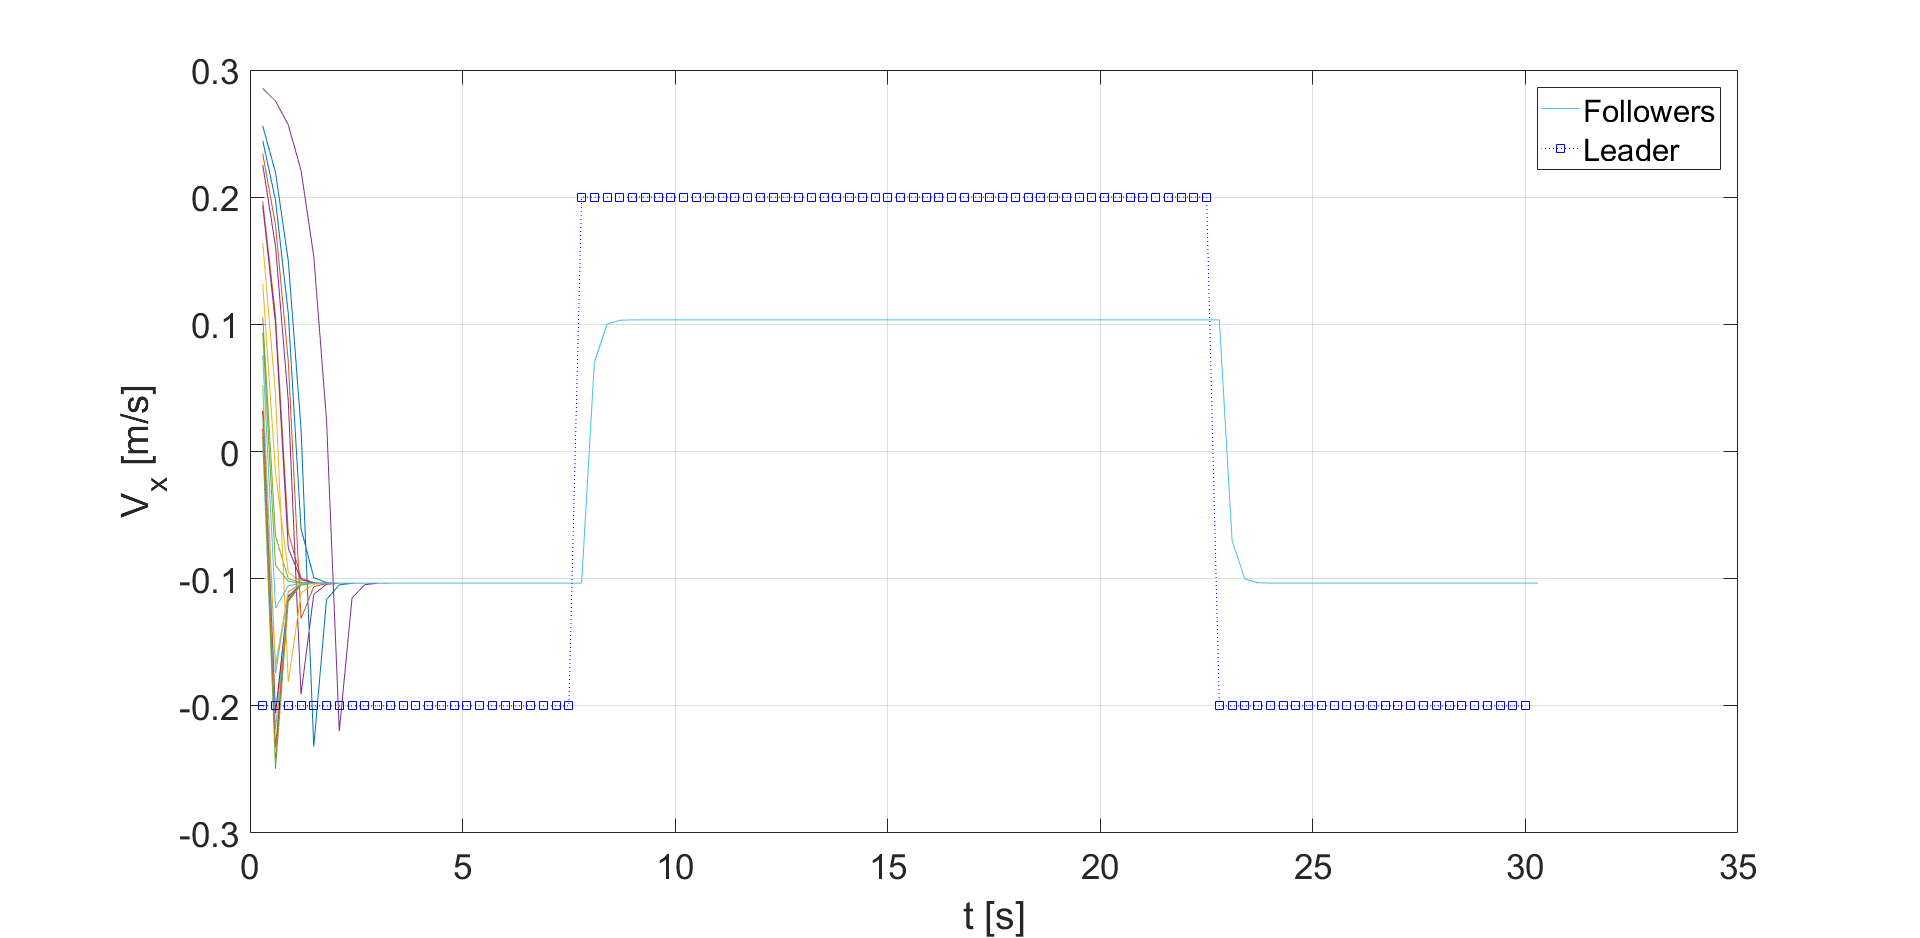
\includegraphics[width=.53\textwidth]{figures/CB_ANTS_Vx.png}
	\centering
	\caption{Velocities in x axis  $V_x$ using CB-ANTS with global measurements.}
	\label{fcbvx}
\end{figure}


According to constant boost force as described in section \ref{cb} the follower robots should align the direction of their velocities with the leader's velocity as depicted in figures \ref{fcbvy}, \ref{fcbvx}. We notice that the followers align to the direction of leader's velocity exponentially fast, even in the beginning of the simulation where they have been assigned with random velocities. On the other hand, the force feedback controller was successfully evaluated as the follower forces converge to the imposed leader's force for both directions as shown in figures \ref{fcbfy}, \ref{fcbfx}.
\begin{figure}[!h]
	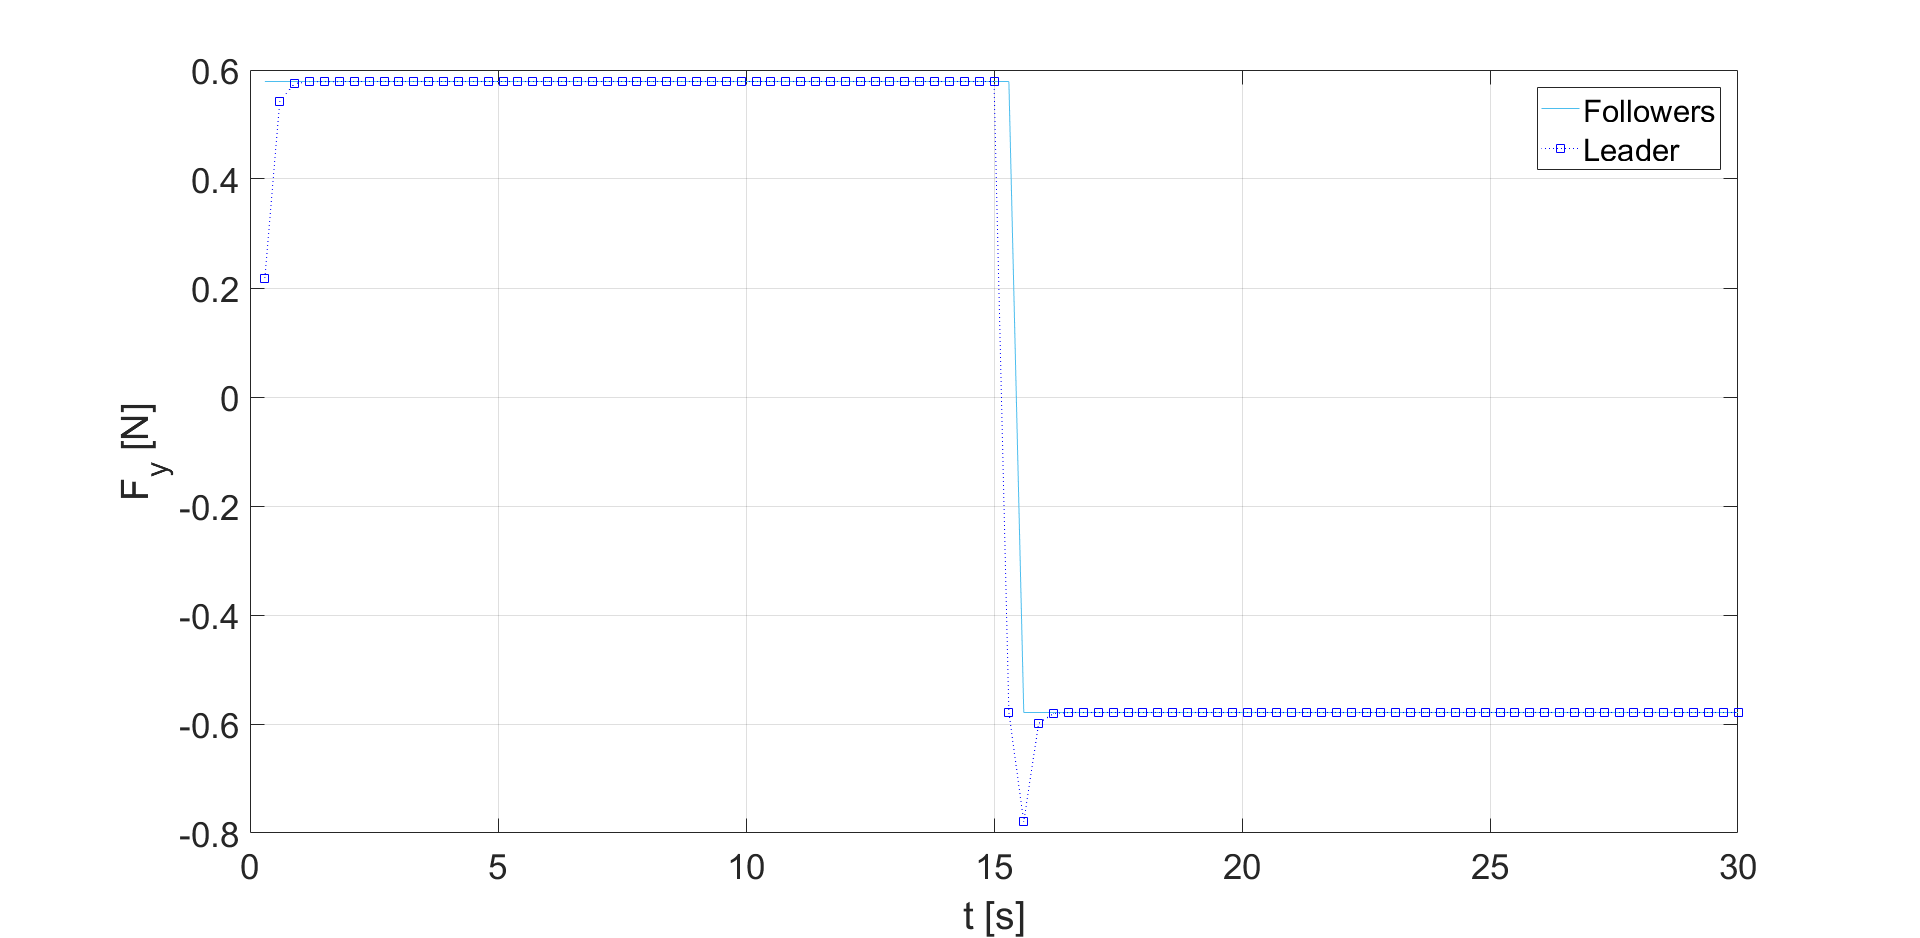
\includegraphics[width=.53\textwidth]{figures/CB_ANTS_Fy.png}
	\centering
	\caption{Forces in y axis $F_y$ using CB-ANTS with global measurements.}
	\label{fcbfy}
\end{figure}
\begin{figure}[!h]
	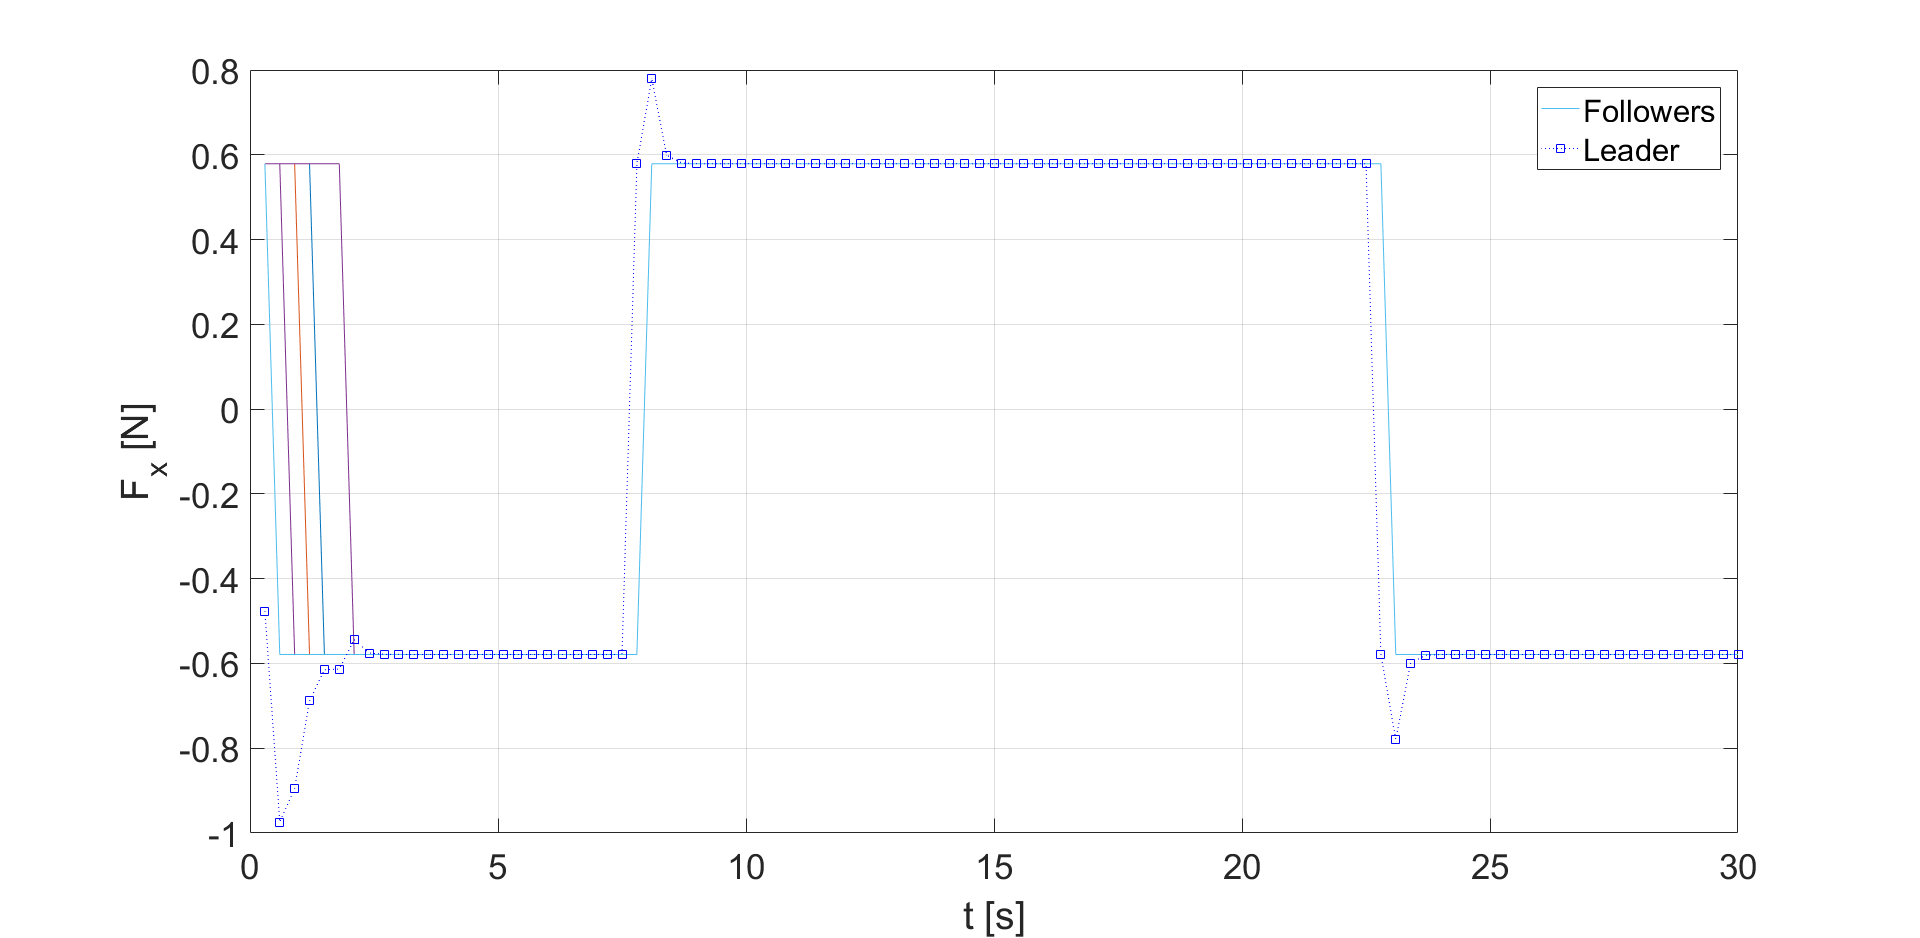
\includegraphics[width=.53\textwidth]{figures/CB_ANTS_Fx.png}
	\centering
	\caption{Forces in x axis $F_x$ using CB-ANTS with global measurements.}
	\label{fcbfx}
\end{figure}


\subsection{P-ANTS Simulations}
For heavyweight objects the proposed methodology was the proportional force (P-ANTS). This technique requires to lift and drag the object on a rolling device where the major type of friction is the rolling friction. The mass of the object that we employed for the simulations was $m=40kg$, the number of robots that took part to the cooperative motion was $N=100$. The maximum applied force of the leader could reach $F_l=0.6N$, while the followers could contribute up to $F_i=0.3N$. The rolling friction was defined to $\mu_v=0.39$, and maximum velocity of the robots up to $v_c=0.3m/s$. The path that was imposed from the leader was a straight line. The developed algorithm was time consuming since for a system of 350 robots and an analysis in both directions the matrices were $700 \times 700$.
\subsubsection{P-ANTS with Global Measurement}
According to proportional force (P-ANTS) as described in section \ref{pants} the follower robots with the force feedback controller converge to the imposed leader's force for both directions as shown in figures \ref{fpfy}, \ref{fpfx}. Moreover, the magnitude of the total forces that was developed on the object is presented in figure \ref{fpsfy}, \ref{fpsfx}. Notice that the leader's force is relatively low in relation with the forces exerted form the follower robots. Thus, the methodology is not evaluated as feasible for a real application as this level of leader's force could even be the noise of the system.
\begin{figure}[!h]
	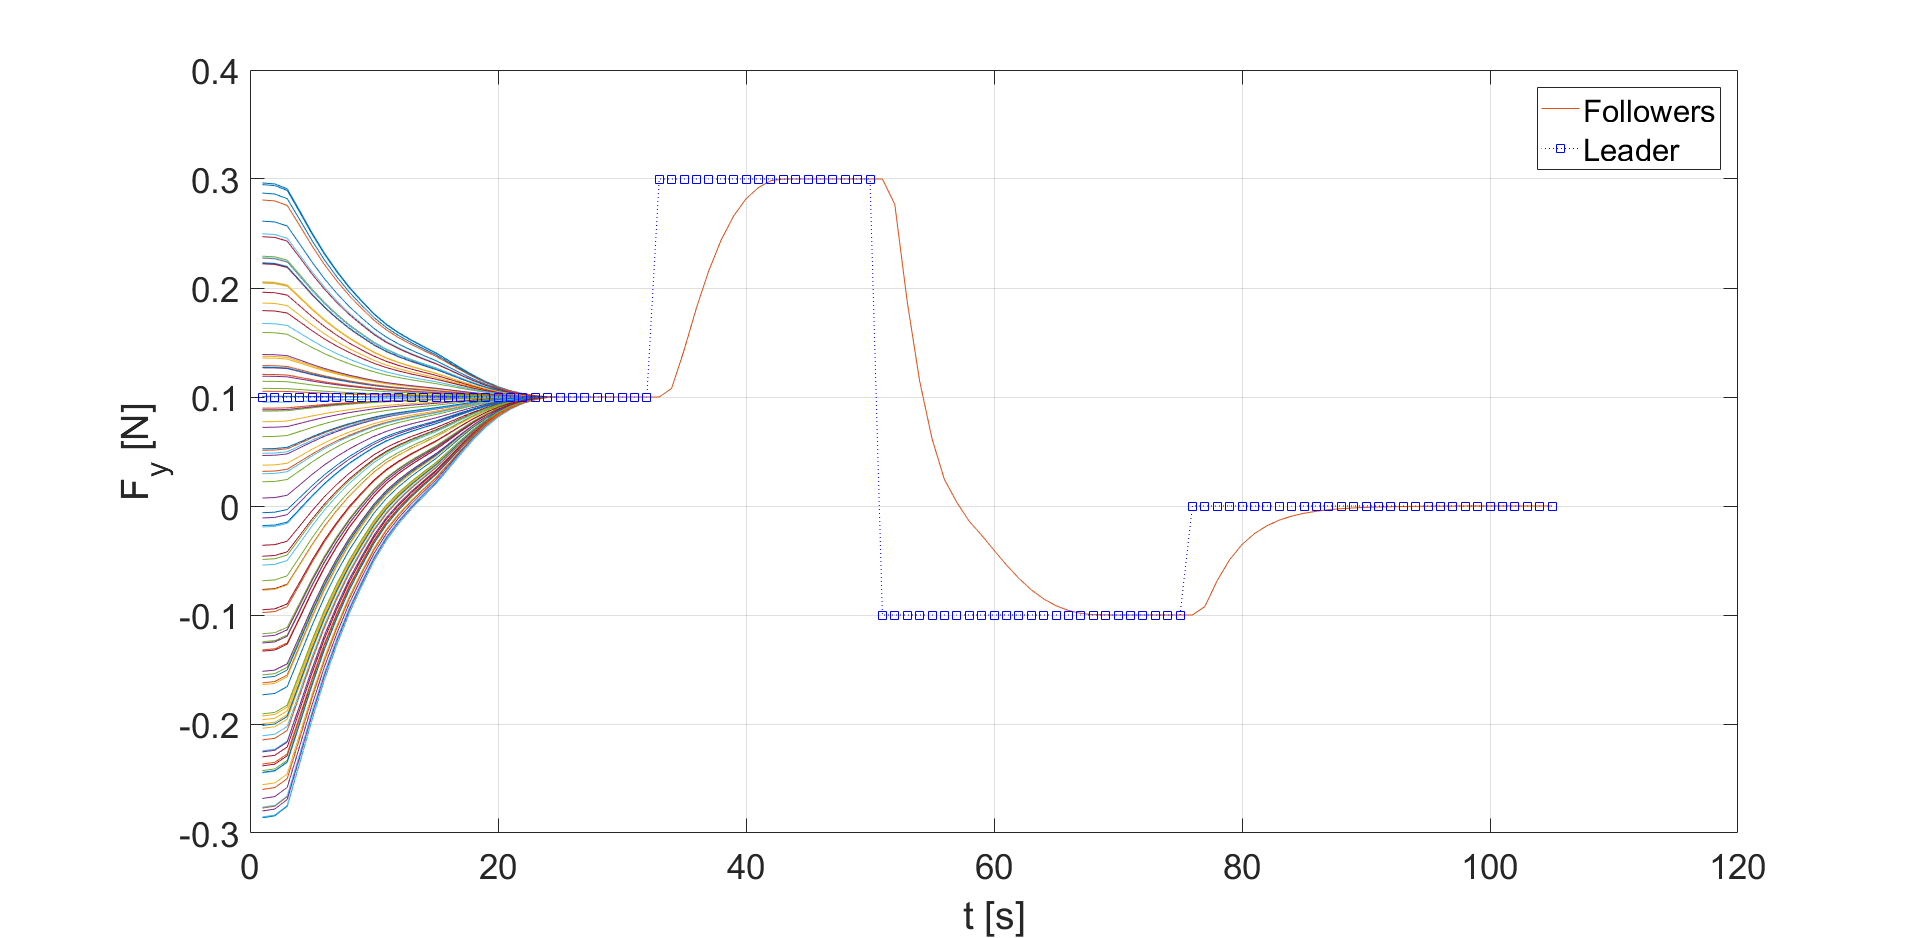
\includegraphics[width=.53\textwidth]{figures/P_ANTS_Fy.png}
	\centering
	\caption{Forces in y axis $F_y$ using P-ANTS with global measurements.}
	\label{fpfy}
\end{figure}
\begin{figure}[!h]
	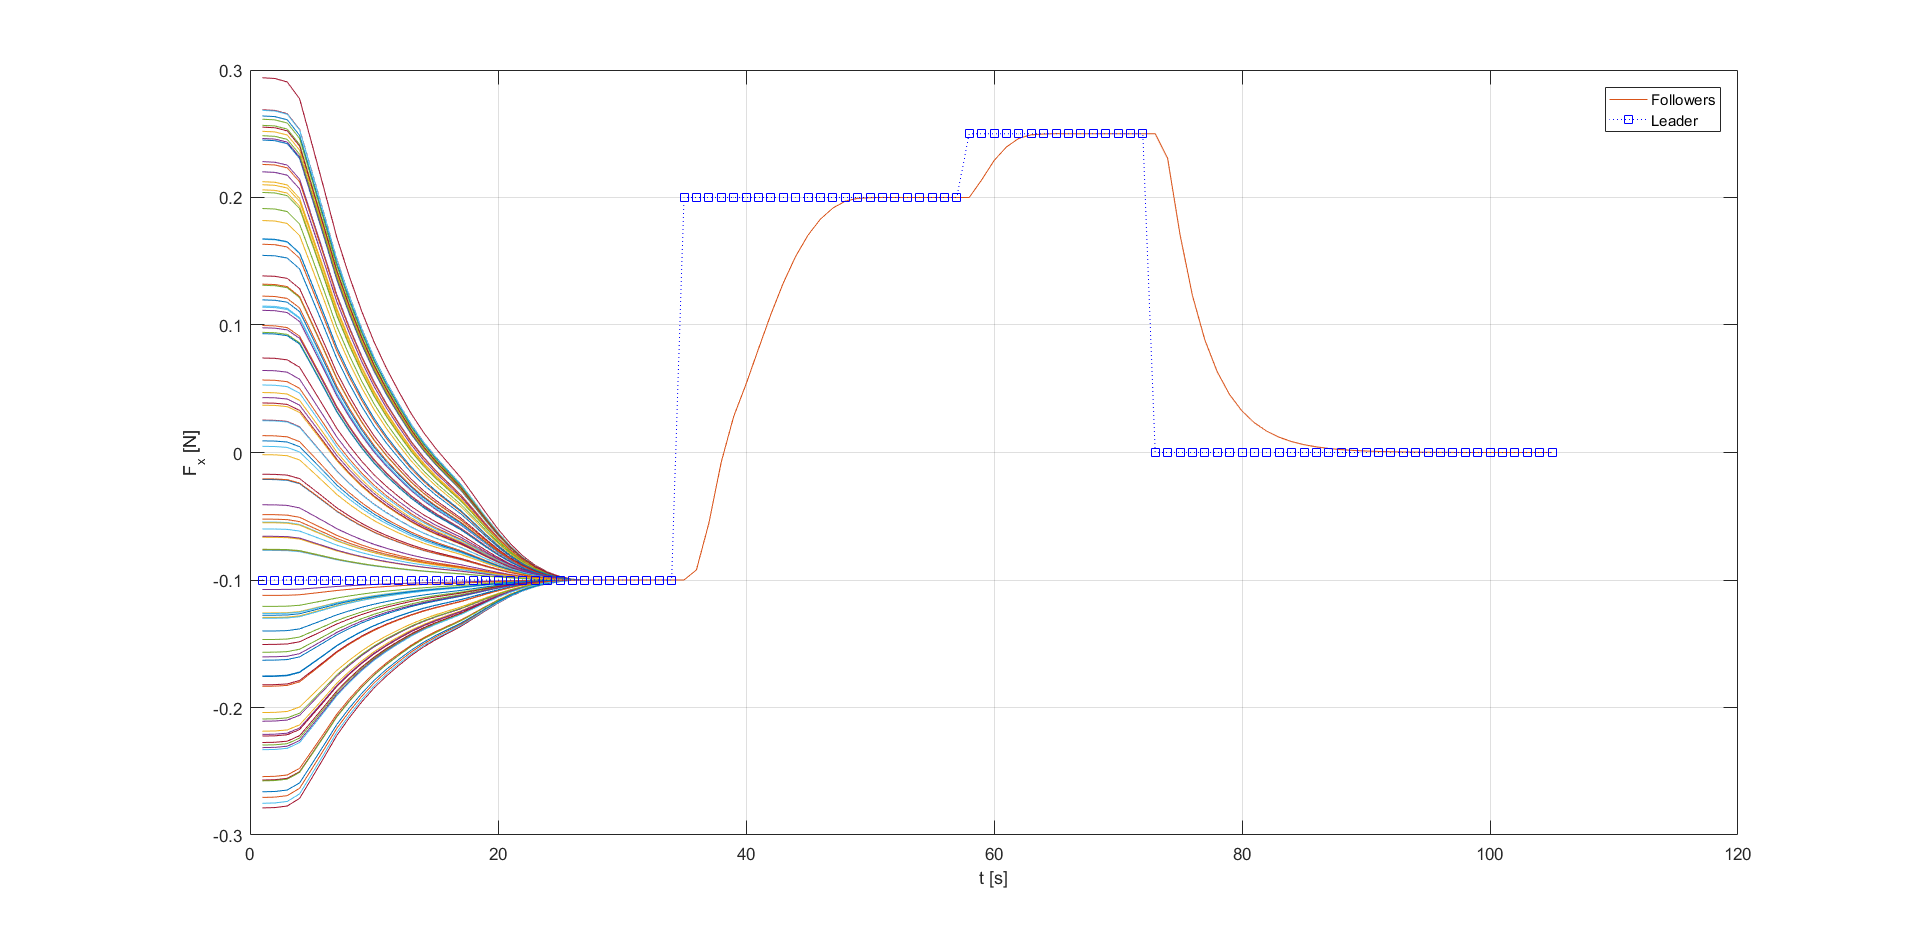
\includegraphics[width=.53\textwidth]{figures/P_ANTS_Fx.png}
	\centering
	\caption{Forces in y axis $F_x$ using P-ANTS with global measurements..}
	\label{fpfx}
\end{figure}

\begin{figure}[!h]
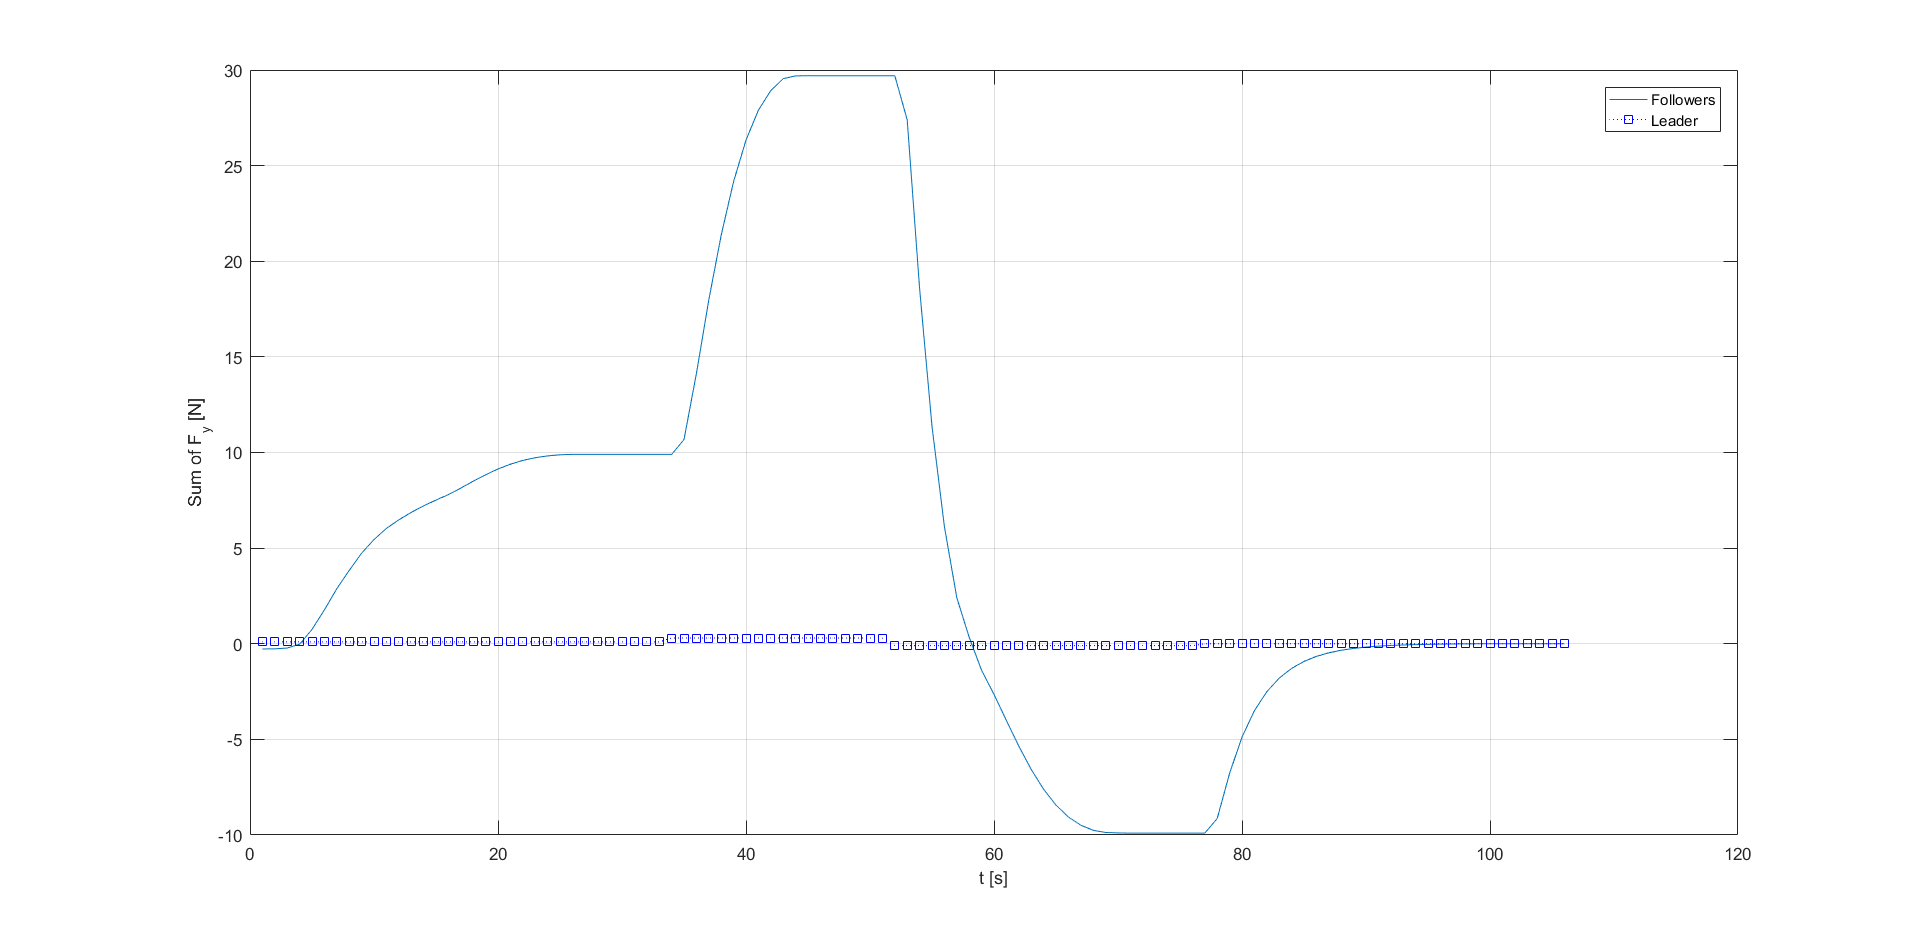
\includegraphics[width=.53\textwidth]{figures/P_ANTS_SumFy.png}
	\centering
	\caption{Sum of forces in y axis $\sum F_y$ using P-ANTS with global measurements.}
	\label{fpsfy}
\end{figure}
\begin{figure}[!h]
	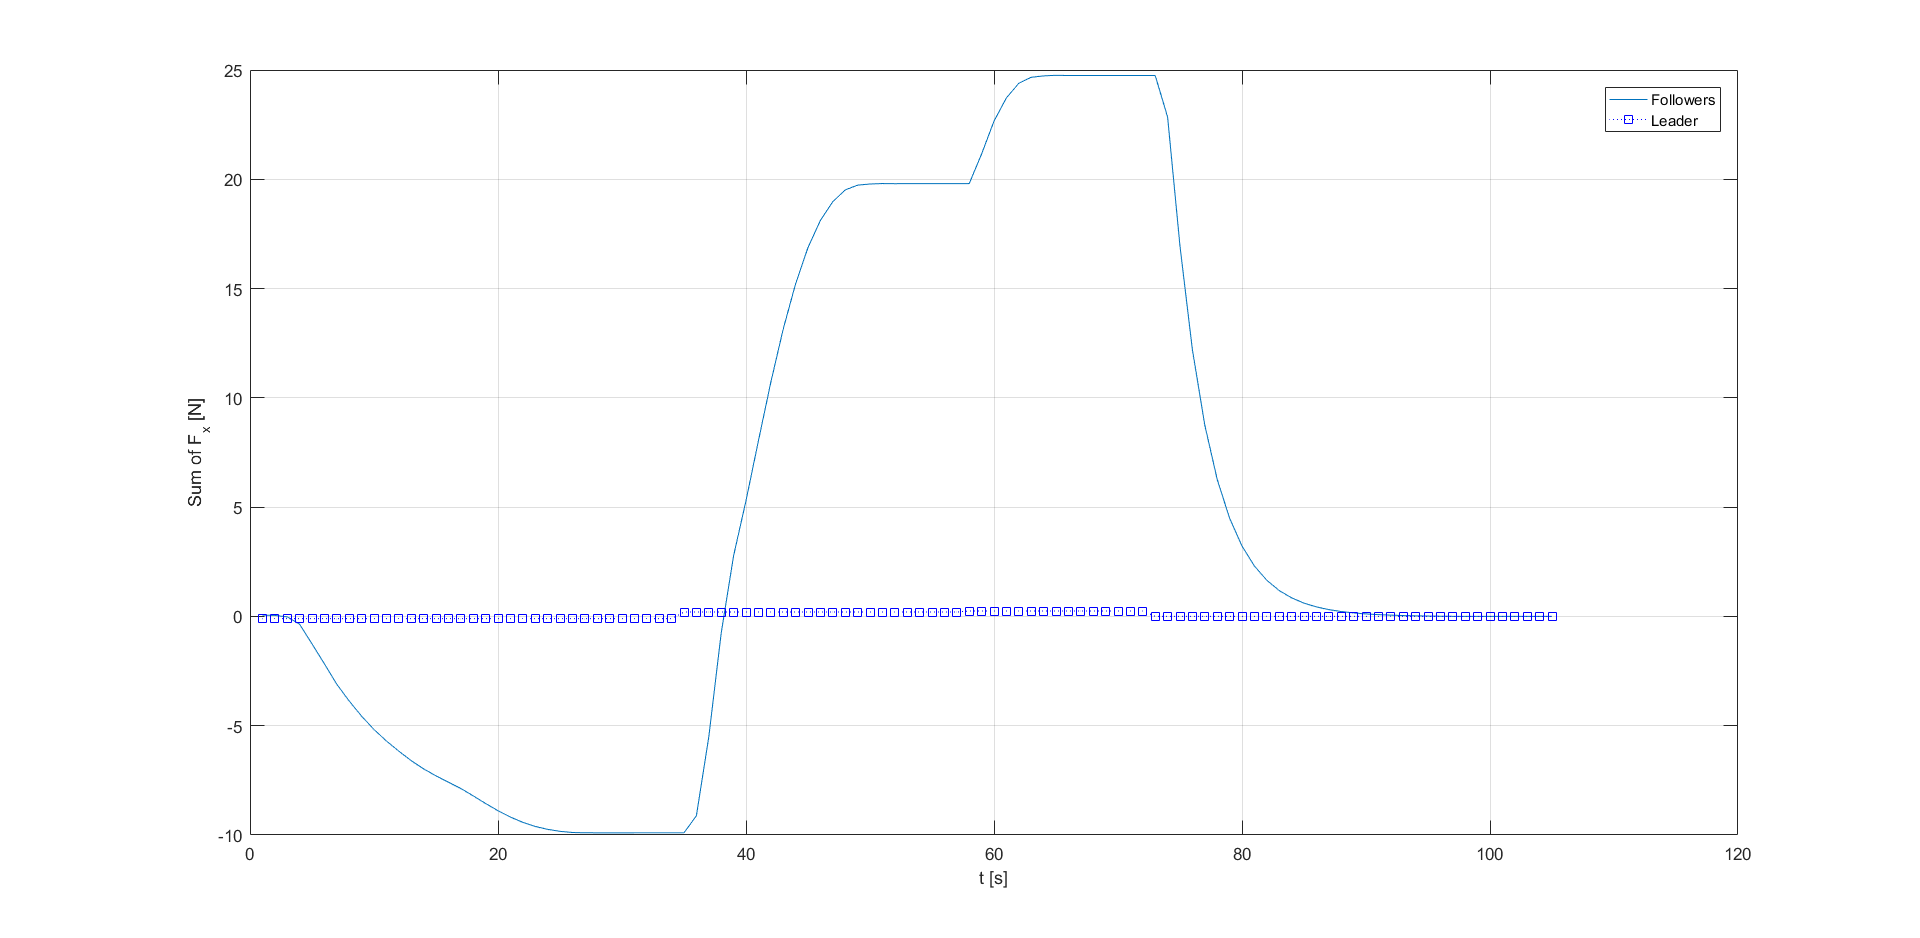
\includegraphics[width=.53\textwidth]{figures/P_ANTS_SumFx.png}
	\centering
	\caption{Sum of forces in x axis $\sum F_x$ using P-ANTS with global measurements.}
	\label{fpsfx}
\end{figure}

\subsubsection{P-ANTS with Local Measurement}
In this set of simulations we employed the proportional force (P-ANTS) algorithm with local information as described in matrix form in equation \ref{mpants}. An important aspect is to carefully select the number of robots, the dimensions of the object, that are related with the moment of inertia, and the mass of the object to assure equation \ref{mpantsBound}.
\begin{figure}[!b]
	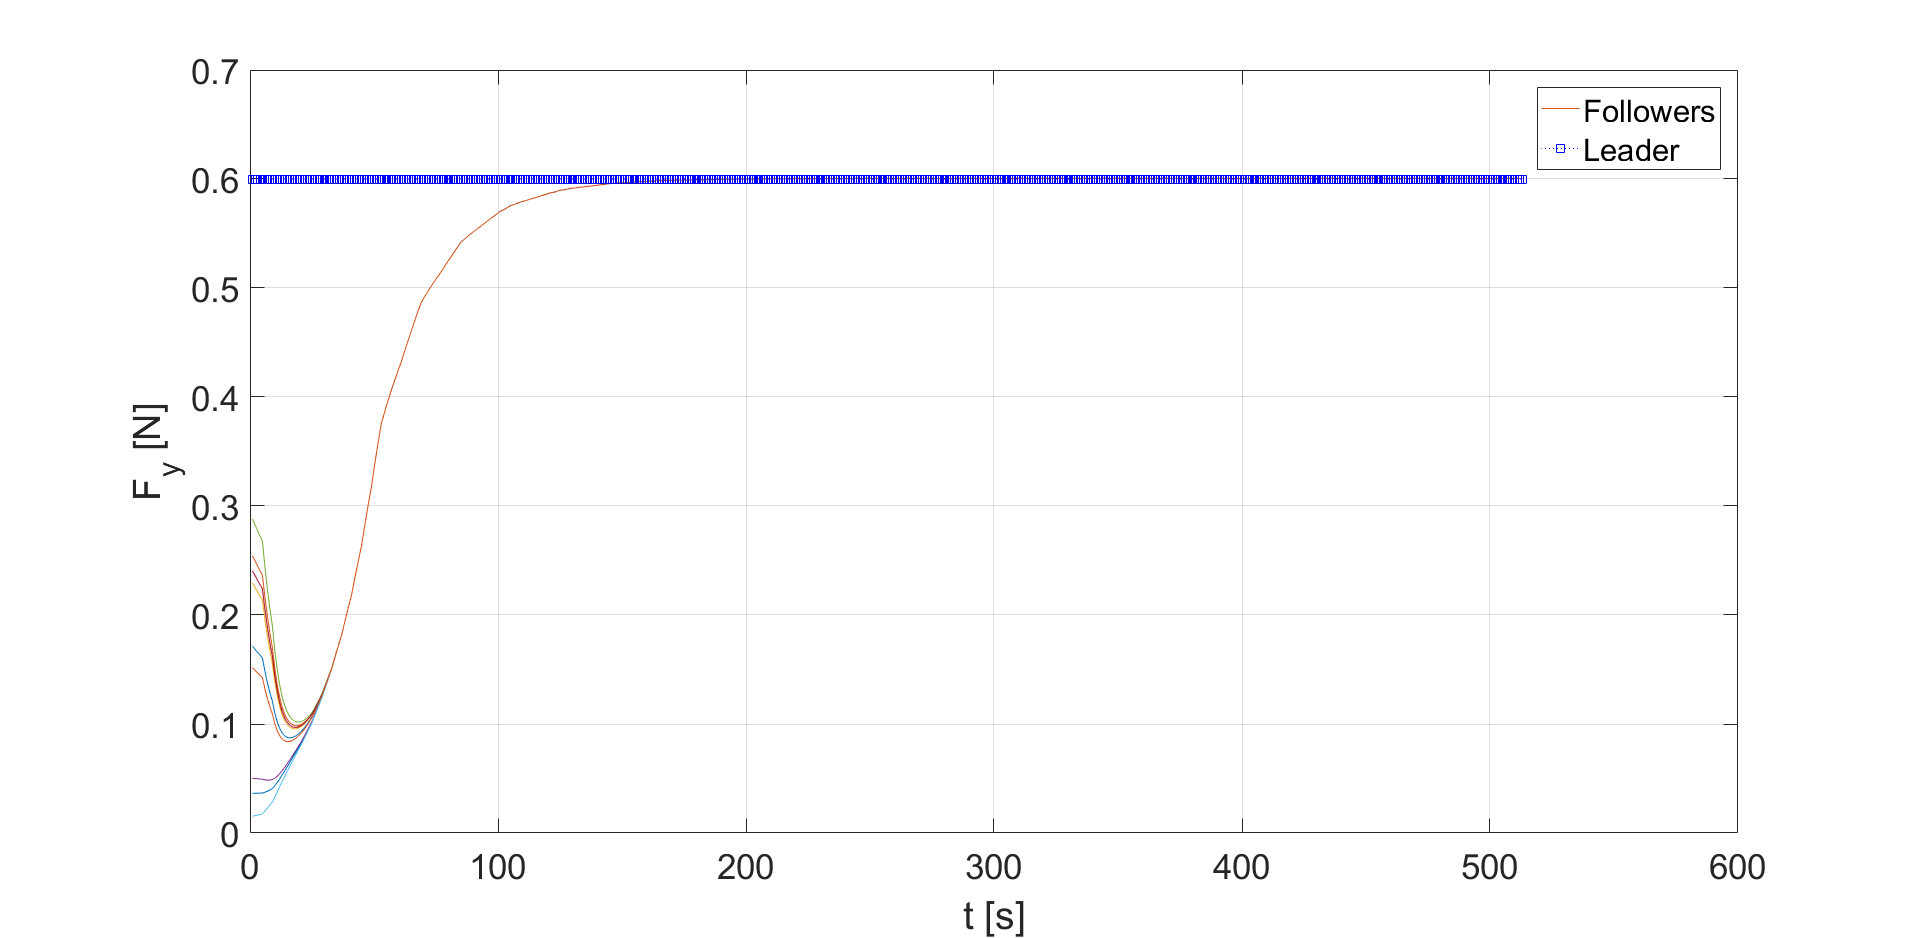
\includegraphics[width=.53\textwidth]{figures/P_ANTS_Local_Fy.png}
	\centering
	\caption{Forces in y axis $F_y$ using P-ANTS with local measurements for 20 robots.}
	\label{fplfy}
\end{figure}
\begin{figure}[!h]
	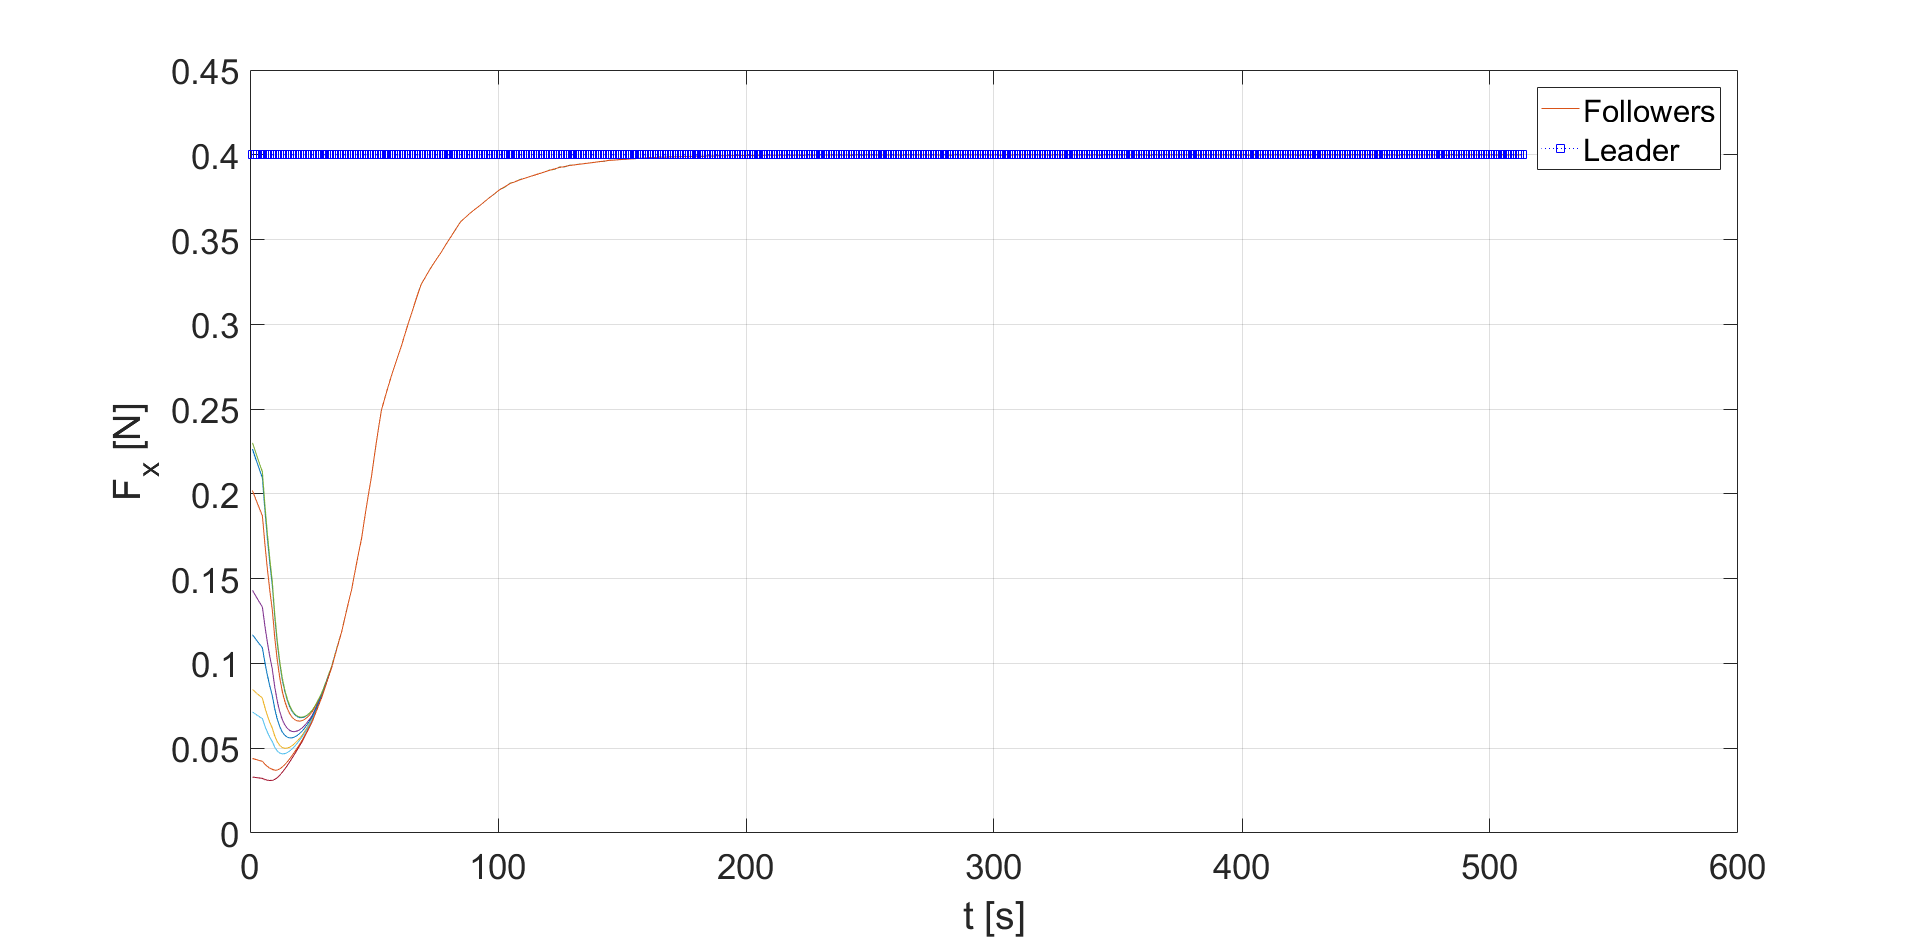
\includegraphics[width=.53\textwidth]{figures/P_ANTS_Local_Fx.png}
	\centering
	\caption{Forces in x axis $F_x$ using P-ANTS with local measurements for 20 robots.}
	\label{fplfx}
\end{figure}
We perform two successful experiments with different number of robots. As mentioned previously the computational requirements of the algorithm is increasing rapidly as the number of robots increases. In both simulation the studied system converged as depicted in figures \ref{fplfy} \ref{fplfx}, but in the second case with 100 robots it took up to 8 hours to finish the calculations \ref{fplfy1}, \ref{fplfx1}.
\begin{figure}[!h]
	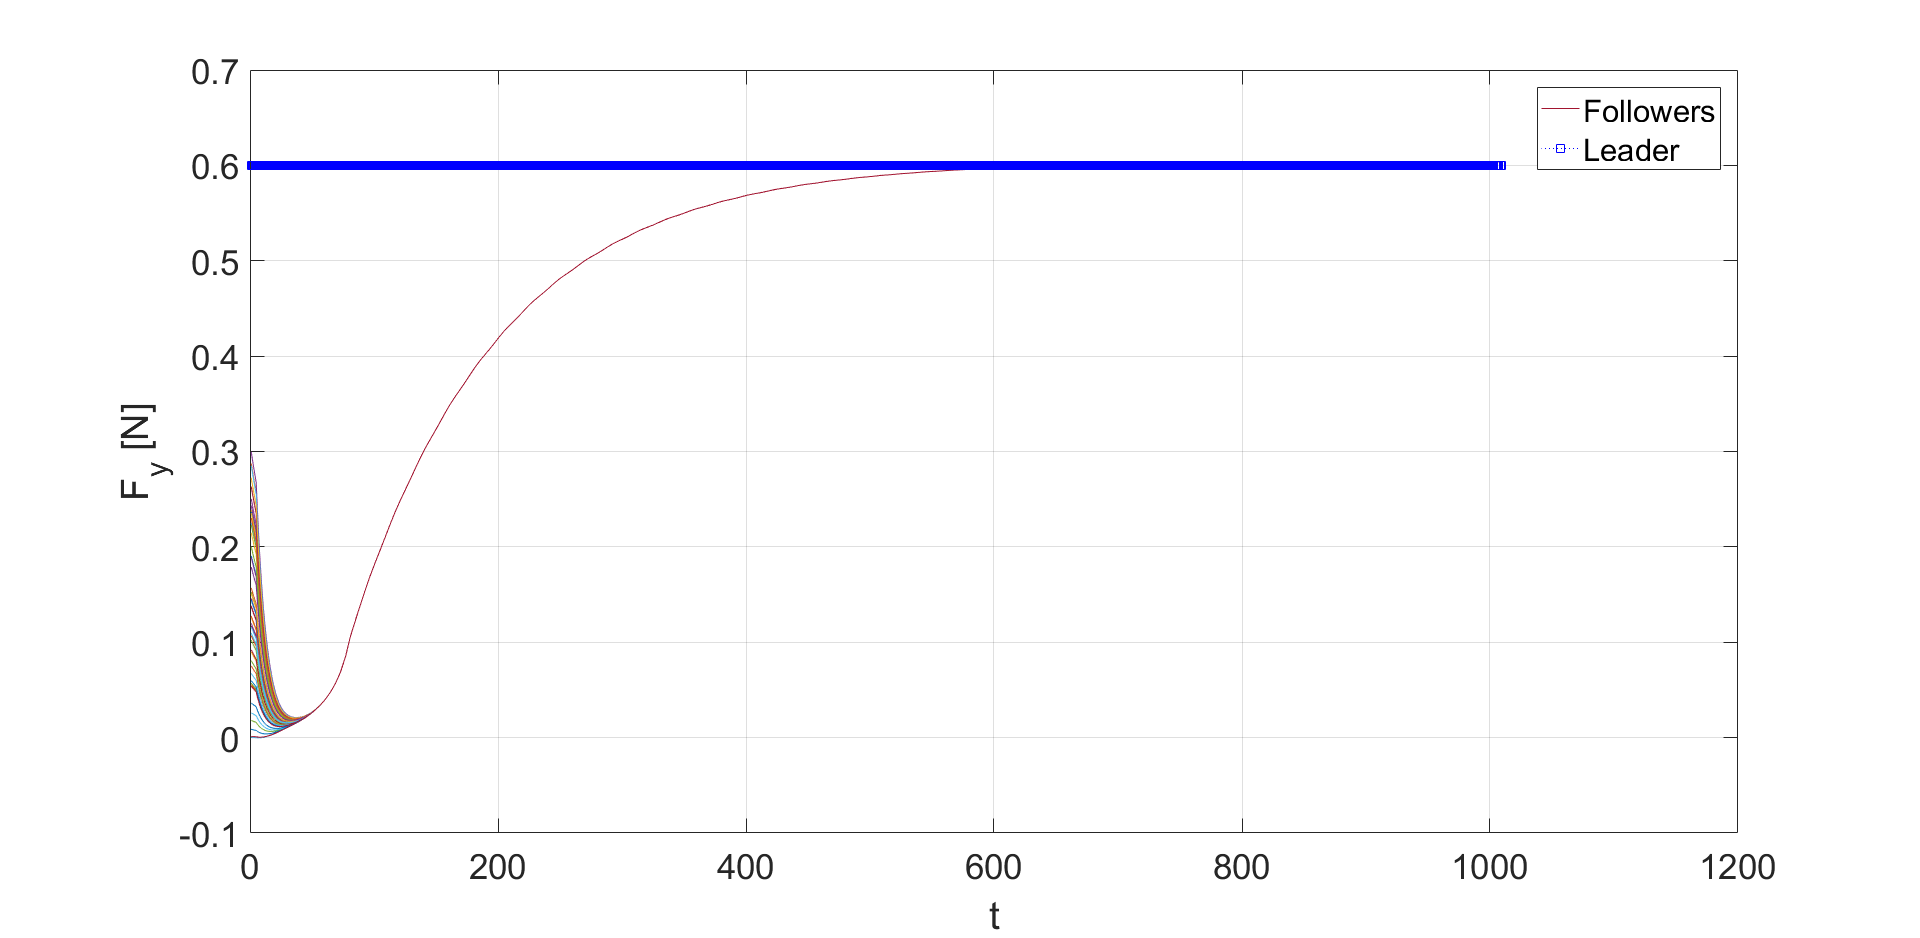
\includegraphics[width=.53\textwidth]{figures/P_ANTS_Local_Fy_100.png}
	\centering
	\caption{Forces in y axis $F_y$ using P-ANTS with local measurements for 100 robots.}
	\label{fplfy1}
\end{figure}
\begin{figure}[!h]
	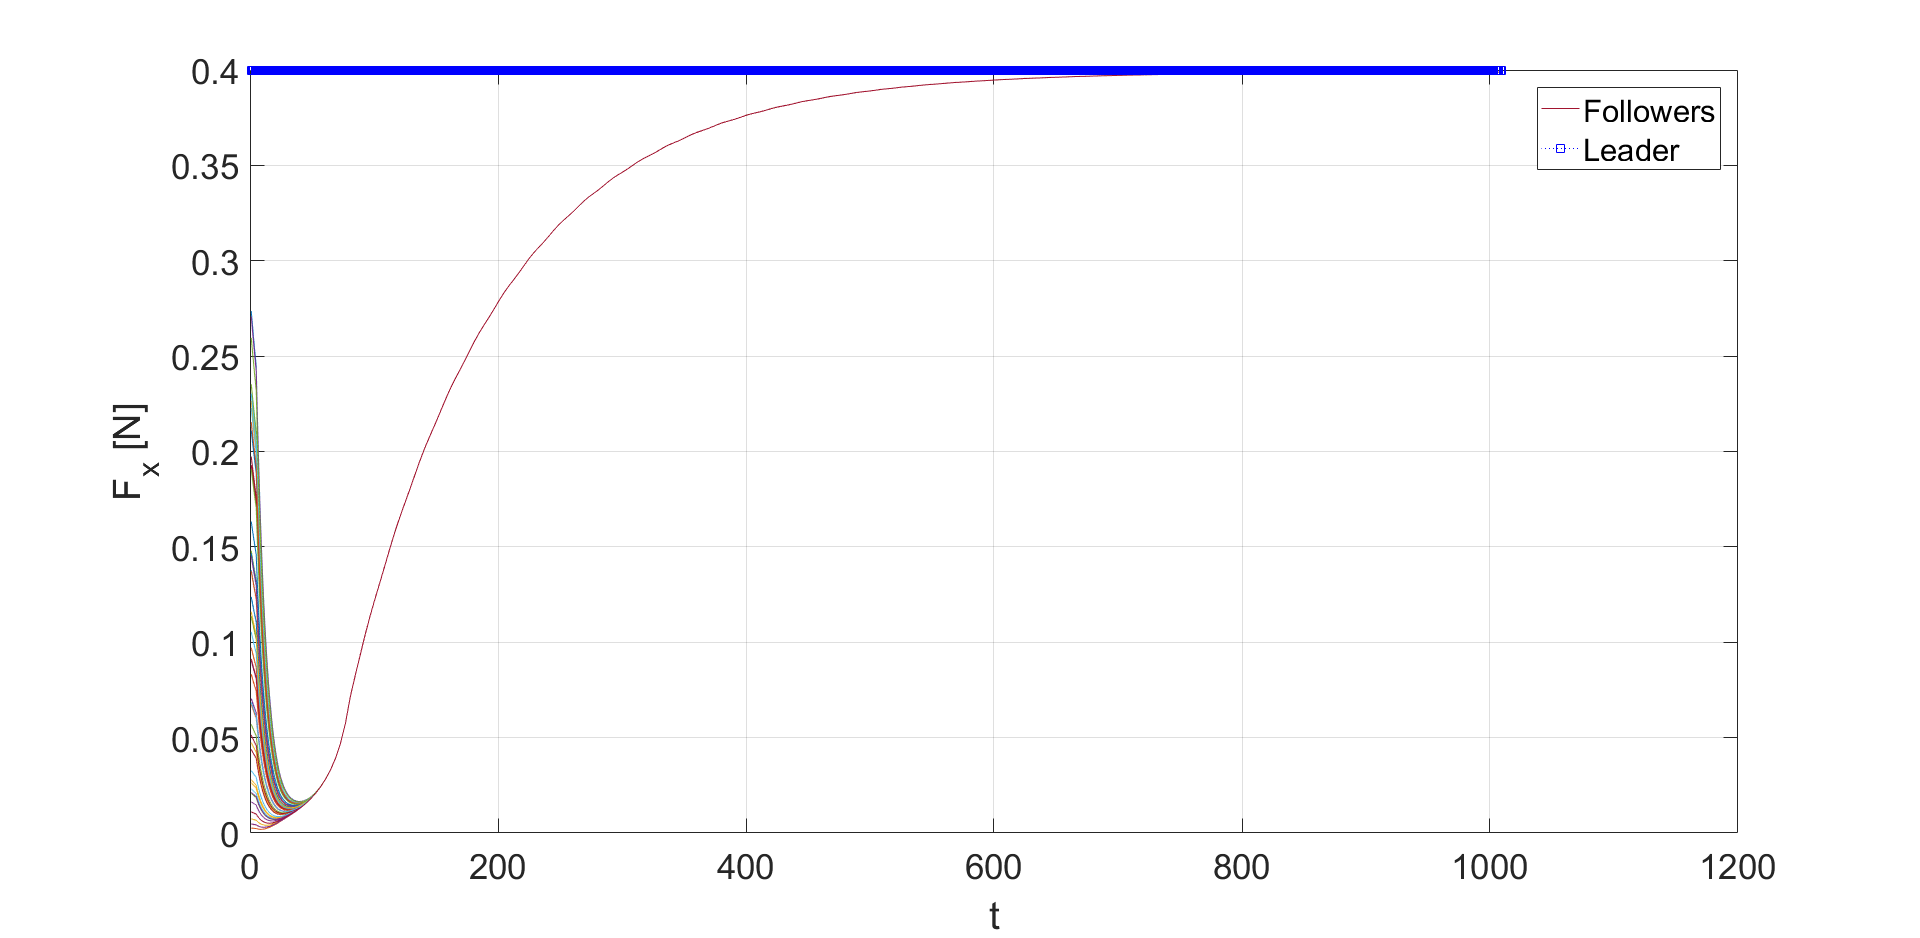
\includegraphics[width=.53\textwidth]{figures/P_ANTS_Local_Fx_100.png}
	\centering
	\caption{Forces in x axis $F_x$ using P-ANTS with local measurements for 100 robots.}
	\label{fplfx1}
\end{figure}


%----------------------------------------------

\section{Conclusions}\label{concl}
In this project a set of cooperative manipulation methodologies without explicit communication was presented. The system operates with force feedback information. Other information are given either locally or provided to the system by external sensors. The leader robot is the only robot that have knowledge about the goal position and the trajectory planning, so it imposes to the follower robots its force intention. Two different cases were analyzed which discriminate the proposed strategy according to the object weight. Constant boost force (CB-ANTS) employed for lightweight objects and the strategy suggests to drag the studied object on the floor. In such case the dominant force is kinetic. The second case deals with heavyweight objects and the strategy propose to lift and place the object on a rolling device. Therefore, the effort of moving the object is less, while the dominant friction in such case is the rolling friction.

Discretizing the object's dynamics ensures an easier analysis, yet study of continuous time system is demanding. Assumptions \ref{as1}, \ref{as2}, \ref{as3} make the methodology compatible only in structured environments. State equations for P-ANTS cannot be employed, because they imply the use of an $N$-Complete graph that requires communication of all agents. An extension of the system in $3D$-space is suggested as the moment of inertia is related with the height of the object.

\bibliographystyle{IEEEtrans}
\bibliography{IEEEabrv,mybib}

\end{document}